% !TeX spellcheck = en
\chapter{Data and Model}
\label{sec:design}
This chapter presents the steps of development and implementation of the proposed approach. The Unity Application for HoloLens was deployed on HMD and a raw data with measures and dimension columns was obtained. This data than was analyzed and preprocessed to ensure that the captured data can be used in corresponding machine learning models. The model architecture was implemented and experimentally improved during training and evaluation steps. 

\section{6-DoF Dataset}
\label{sec:design:dataset}
This section describes how the dataset was obtained, analyzed and presents the visualization of user's head position and rotation. The real 6-DoF dataset must be used as training data from which the model can learn the spacial and time dependences. This step is crucial for a high accuracy prediction and almost all machine learning approaches requires not only row data collection but also data exploration and data preprocessing steps to be done before training begins.

\subsection{Data collection from HMD}
\label{sec:design:dataset:HL}
In this master thesis HoloLens 2, the second iteration of Microsoft's head-mounted mixed reality device, was used for data collection. The user position and orientation were obtained with Unity application developed for this purpose. Main Camera in Unity is automatically configured to track head movements. More details about Unity application can be found in section \ref{sec:imp:programming:unity}.\\
Using the Main Camera, a user position $(x, y, z)$ and orientation in quaternion $(qx, qy, qz, qw)$ were logged in a $csv$-file. Quaternions obtained from HMD will be used to define a rotation by four numbers. Quaternions representations are very convenient for operations such as composition or rotations and coordinate transformation \cite{principles_robot_motion_book}. For these reasons quaternions are chosen for the representation of user head's rotation in three dimensions. Comparing to dataset in \cite{serhan_kalman}, the additional parameters were recorded from the Main Camera in order to add more information during training processes. Thus the world-space speed of the camera in meters per second was recorded. Unity velocity has the speed in $(x, y, z)$ defining the direction. The obtained 6-DoF dataset has 10 features used in training process: position $(x, y, z)$, orientation  $(qx, qy, qz, qw)$ and velocity $(x, y, z)$.\\
The datasets were recorded in the laboratory space. HMD was presented to users and the basic functions were explained. During data recording, users freely walked wearing HMD in laboratory space. The Unity application, running on HMD, not only recorded the mentioned before parameters but also had a volumetric animated object placed placed 3 meters ahead of the user in the Mixed Reality environment. No personal data was recorded during these sessions and all traces are obtained anonymously. Thus, after an Unity application was launched, user could immediately see the animated object. The several traces were recorded at least for 10 minutes each. It allows to have enough data after splitting the dataset into training, test and validation partitions. Table \ref{tab:raw_data} show the first 20 rows from raw dataset obtained from HoloLens 2 and used in training. As mentioned above, 6-DoF dataset has 10 columns, thus the table \ref{tab:raw_data} presents only $timestamp$ and position $(x, y, z)$ columns. 

\begin{table}[!ht]
		\footnotesize
		\centering
	\begin{tabular}{|l|l|l|l|}
		\hline
		timestamp & x & y & z \\ [0.5ex] 
		\hline\hline
		2.649431 & 0.004954389 & 0.003402365 & 0.01010712 \\ \hline
		2.66943 & 0.00459053 & 0.003120769 & 0.01130438 \\ \hline
		2.698009 & 0.003960807 & 0.002990472 & 0.01276976 \\ \hline
		2.719285 & 0.003730714 & 0.003037783 & 0.01305151 \\ \hline
		2.746641 & 0.003252693 & 0.003489003 & 0.01368421 \\ \hline
		2.764094 & 0.003153284 & 0.003518121 & 0.01400959 \\ \hline
		2.780033 & 0.003087142 & 0.003409061 & 0.01435899 \\ \hline
		2.802086 & 0.003021815 & 0.00314023 & 0.01473305 \\ \hline
		2.815575 & 0.002789935 & 0.003551113 & 0.01506916 \\ \hline
		2.832602 & 0.002527435 & 0.003542757 & 0.01534094 \\ \hline
		2.848514 & 0.002212256 & 0.003605011 & 0.01565307 \\ \hline
		2.863769 & 0.001921757 & 0.003369405 & 0.01590317 \\ \hline
		2.879648 & 0.001668522 & 0.00348538 & 0.01607716 \\ \hline
		2.89686 & 0.001501704 & 0.003624826 & 0.01627397 \\ \hline
		2.913541 & 0.001487849 & 0.00359472 & 0.01643924 \\ \hline
		2.930006 & 0.001501501 & 0.003769569 & 0.01669565 \\ \hline
		2.948201 & 0.001617525 & 0.004252479 & 0.01697758 \\ \hline
		2.964302 & 0.001755987 & 0.004224311 & 0.01721937 \\ \hline
		2.97978 & 0.001838901 & 0.004487753 & 0.01747578 \\ \hline
		2.997117 & 0.002005509 & 0.005007531 & 0.01782864 \\ \hline
	\end{tabular}
\caption{\label{tab:raw_data}Raw data from HoloLens 2}
\end{table}

The first column in dataset is $timestamp$. It is obviously, that timestamp appears in row dataset not linearly and comes with different pauses. Even the high-cost HMD, like used in this research HoloLens 2, is sometimes unstable in frame rate during collecting data\footnote{https://docs.microsoft.com/en-us/windows/mixed-reality/develop/advanced-concepts/hologram-stability}.  In the Unity Application, the frame rate is  60 Hz which means that data will be collected per 0.016(6) second. Unfortunately, HMD could have delays, and the time gap of two samples may be reduced or increased, as we can observe on raw dataset. Data on some expected timestamps may be unavailable in HMS for recording. Those sequences with fewer timesteps may be considered to have missing values. To deal with above situation, the preprocessing steps must be done. They are described in a section \ref{sec:design:dataset:preprocessing} below. 

\subsection{Data preprocessing}
\label{sec:design:dataset:preprocessing}
As was mentioned in section \ref*{sec:design:dataset:HL}, the raw sensor data obtained from the HoloLens was unevenly sampled at 60 Hz and had different temporal distances between consecutive samples. \textit{Gül et al., 2020} obtained the similar raw dataset from same HMD and interpolated it to obtain temporally equidistant samples. Same as it was done in work \cite{serhan_kalman}, the position and velocity data were upsampled using linear interpolation and for quaternions SLEP was used. During preprocessing step Euler angles (yaw, pitch, roll) were calculated from quaternions and these parameters are used for visualization purposes. Although the interpolated $csv$-file contains additional Euler angles columns, only described in section \ref{sec:design:dataset:HL} parameters were used for training and prediction. The table \ref{tab:inter_data} lists first 20 rows for columns $timestamp$ and position $(x, y, z)$ from interpolated dataset. This interpolated dataset is created with linear interpolation and SLEP mathematical methods from raw dataset shown in table \ref{tab:raw_data}. 

\begin{table}[!ht]
	\footnotesize
	\centering
	\begin{tabular}{|l|l|l|l|}
		\hline
		timestamp & x & y & z \\ [0.5ex] 
		\hline\hline
		0.0 & 0.004954389 & 0.003402365 & 0.01010712 \\ \hline
		5000000.0 & 0.004833102666666667 & 0.0033084996666666667 & 0.010506206666666667 \\ \hline
		10000000.0 & 0.004711816333333333 & 0.0032146343333333332 & 0.010905293333333333 \\ \hline
		15000000.0 & 0.00459053 & 0.003120769 & 0.01130438 \\ \hline
		20000000.0 & 0.004485576166666666 & 0.003099052833333333 & 0.011548609999999999 \\ \hline
		25000000.0 & 0.004380622333333333 & 0.0030773366666666667 & 0.011792839999999999 \\ \hline
		30000000.0 & 0.0042756685 & 0.0030556205 & 0.01203707 \\ \hline
		35000000.0 & 0.004170714666666667 & 0.003033904333333333 & 0.0122813 \\ \hline
		40000000.0 & 0.004065760833333334 & 0.003012188166666667 & 0.01252553 \\ \hline
		45000000.0 & 0.003960807 & 0.002990472 & 0.01276976 \\ \hline
		50000000.0 & 0.00390328375 & 0.00300229975 & 0.0128401975 \\ \hline
		55000000.0 & 0.0038457605 & 0.0030141275 & 0.012910635 \\ \hline
		60000000.0 & 0.00378823725 & 0.00302595525 & 0.0129810725 \\ \hline
		65000000.0 & 0.003730714 & 0.003037783 & 0.01305151 \\ \hline
		70000000.0 & 0.0036510438333333334 & 0.0031129863333333335 & 0.01315696 \\ \hline
		75000000.0 & 0.003571373666666667 & 0.003188189666666667 & 0.01326241 \\ \hline
		80000000.0 & 0.0034917035000000003 & 0.003263393 & 0.01336786 \\ \hline
		85000000.0 & 0.0034120333333333332 & 0.0033385963333333333 & 0.01347331 \\ \hline
		90000000.0 & 0.0033323631666666667 & 0.0034137996666666667 & 0.01357876 \\ \hline
		95000000.0 & 0.003252693 & 0.003489003 & 0.01368421 \\ \hline
	\end{tabular}
	\caption{\label{tab:inter_data}Interpolated data from HoloLens 2}
\end{table}


After the interpolated dataset was plotted as figure \ref{fig:inter_data}, the important observations based on the sample trace could be done. While the user position data plots look appropriate for machine learning algorithms, the two graphs with orientation show data that is not the perfect case for usage with machine learning technologies and could decrease the prediction rate. The real part $qw$ and the component $qy$ of quaternion and $yaw$ of Euler angles are obviously discontinuous making it hard for a predictor to learn. A orientation on quaternions is used in training, thus this data requires a few additionally preprocessing steps. Usually, when doing calculation with quaternions, quaternions must be normalized to a unit length in order to represent valid rotations \cite{principles_robot_motion_book}. The normalized quaternion can be calculated using formula:
\begin{equation}
U_g = \frac{q}{|| q ||} = \frac{w}{|| q ||} + i \cdot \frac{x}{|| q ||} + j \cdot \frac{y}{|| q ||} + k \cdot \frac{z}{|| q ||}
\end{equation}

where $|| q || $ is a magnitude and can be found with formula:
\begin{equation}
|| q || = \sqrt{w^2 + x^2 + y^2 + z^2 }
\end{equation}

During experiments with quaternions in dataset obtained from HoloLens was found that quaternion magnitudes $|| q ||$ in HoloLens dataset are equal to 1. Thus data came from HMD already normalized, so that a quaternion in dataset kept the same orientation as it was during user's movement but its magnitude is 1.0.


\begin{figure}[htb]
	\begin{center}
		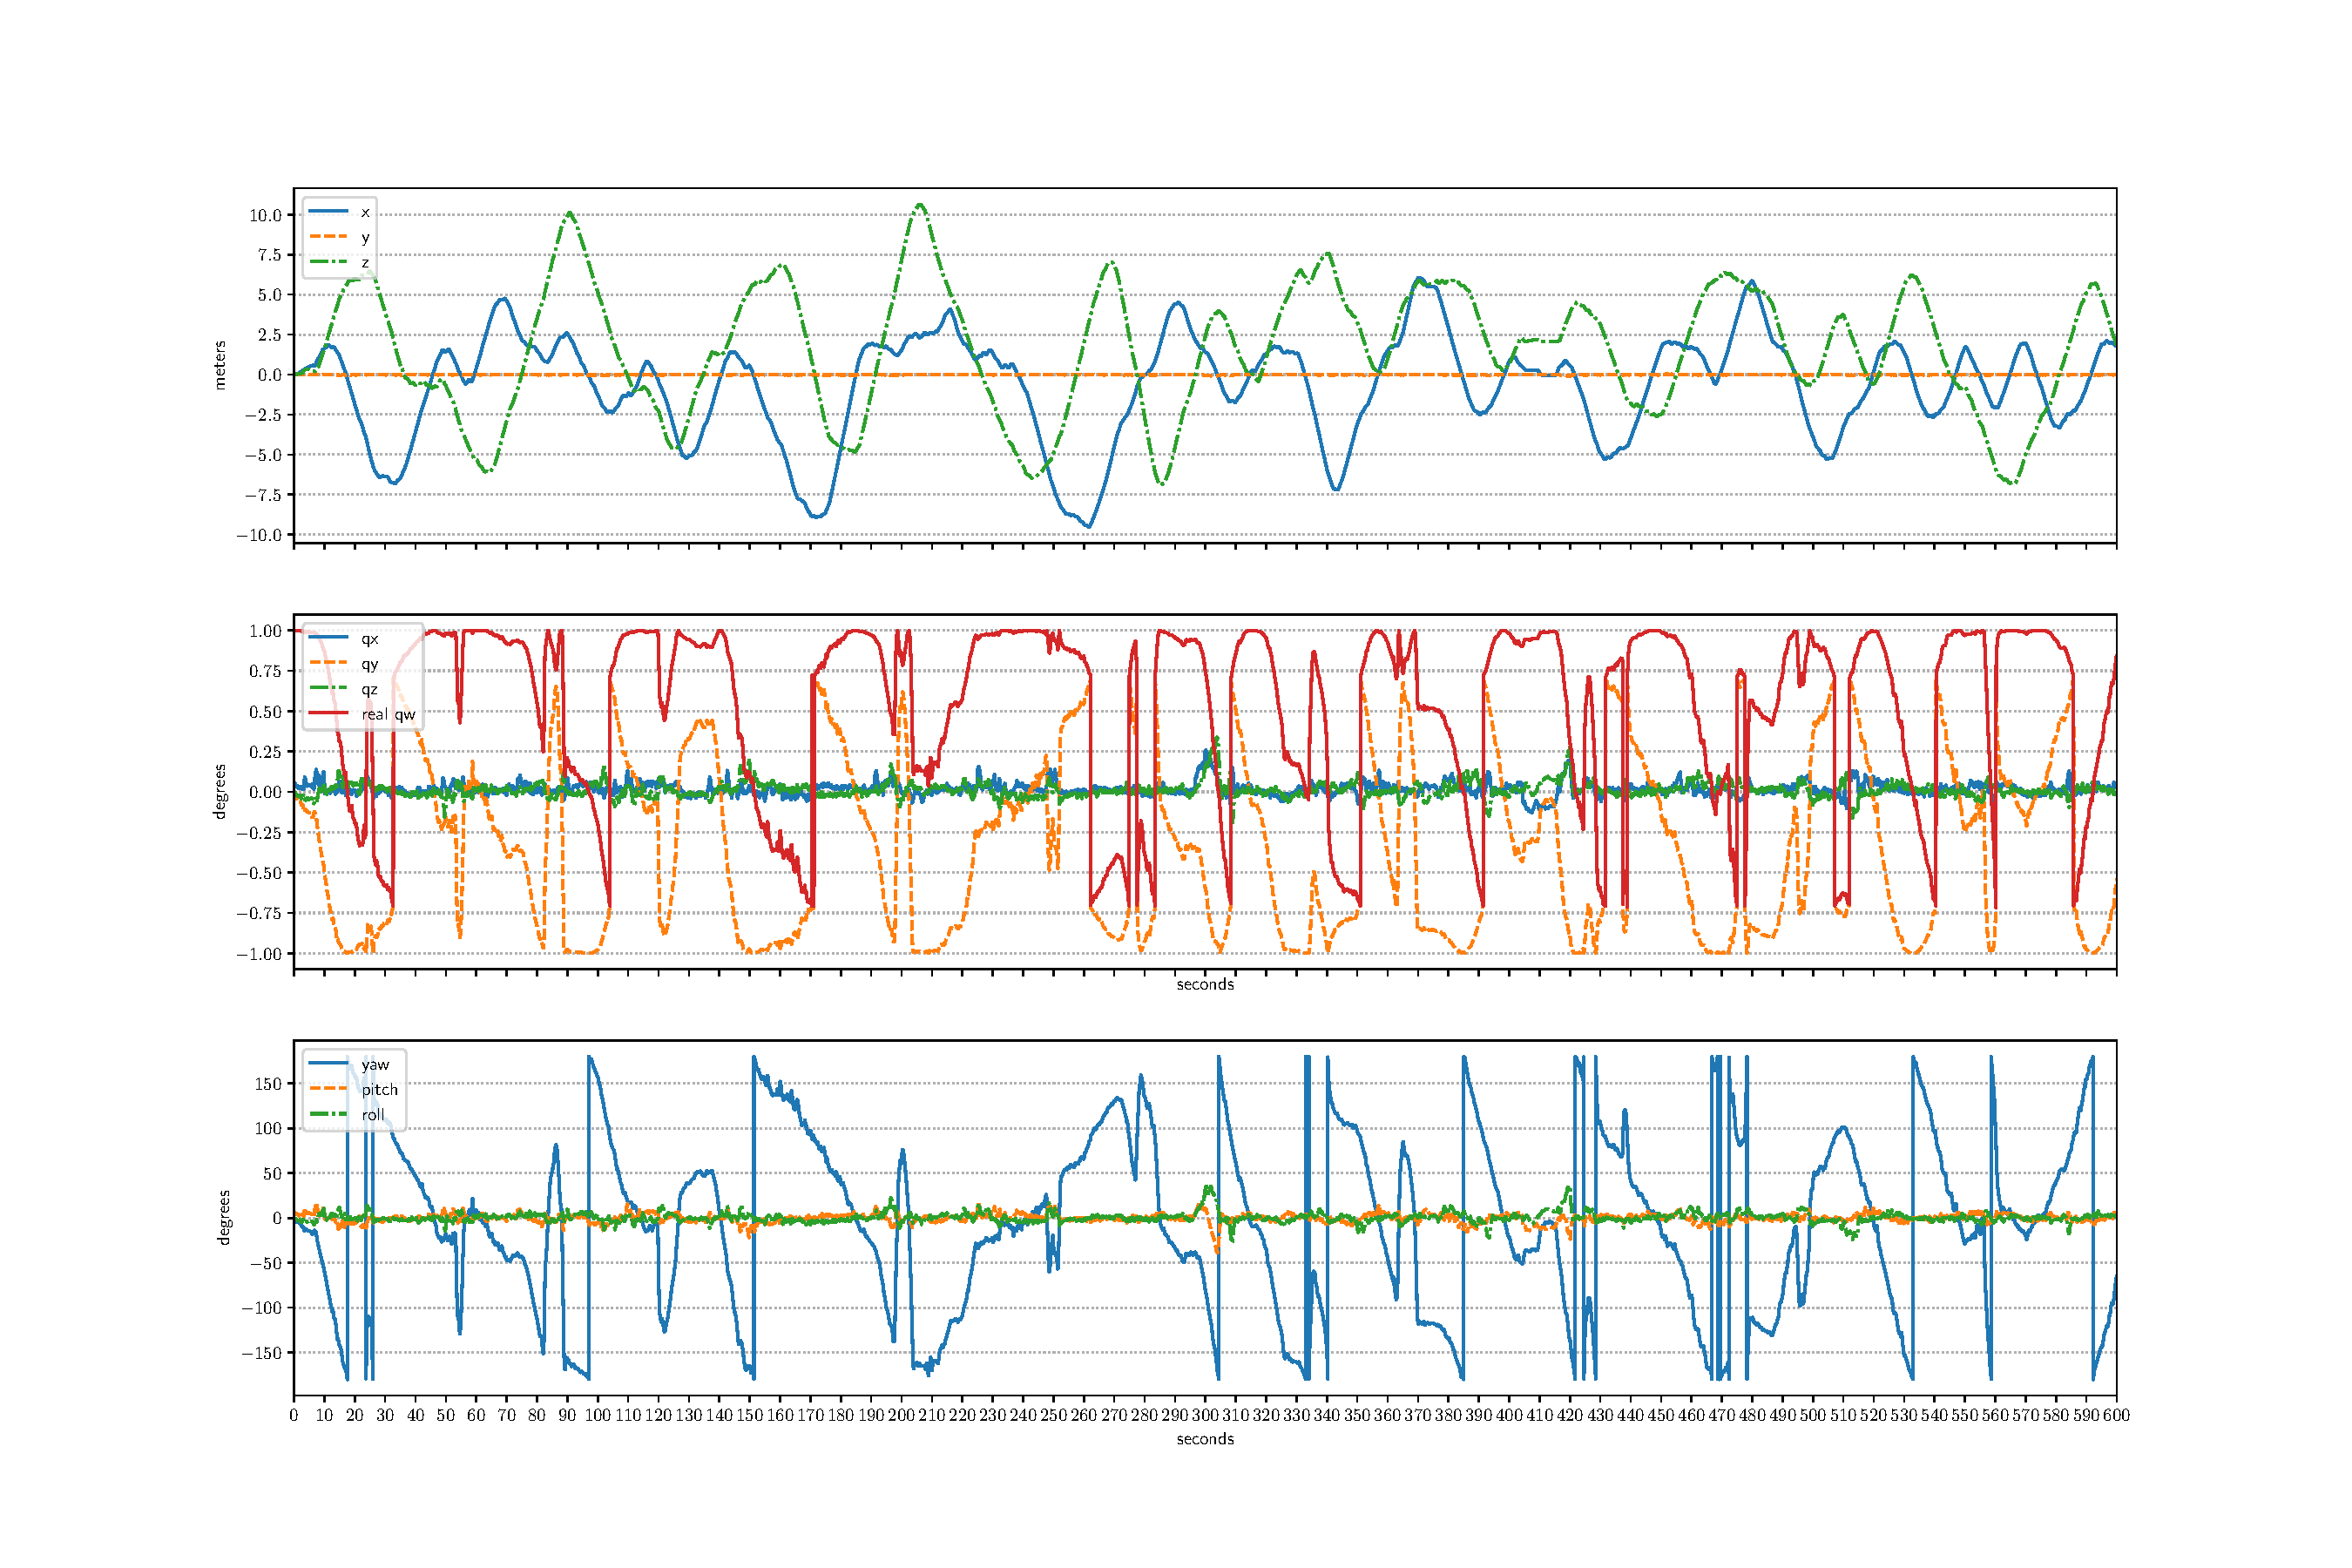
\includegraphics[width=1\textwidth, keepaspectratio]{gfx/Fig-1556-interpolated.pdf}
		\caption{\label{fig:inter_data}Interpolated 6-DoF dataset's user position and orientation in quaternions and Euler angles.}
	\end{center}
\end{figure}

Next, quaternions between neighboring points in obtained dataset represent the very similar orientation made by user wearing HMD step by step. The middle plot on figure \ref{fig:norm_data} has discontinuities that can be seen on $qw$ line. But regardless the discontinuity (sharp change of line from negative to positive area with the same amplitude) the two neighboring quaternions with similar rotation have significant 4D vector space between them. It makes prediction worse what can be proved by RMSE and MSE rotation metrics. Flipping the sign will not affect the rotation, but it will ensure that there are no large jumps in 4D vector space when the rotation difference in rotation space (SO(3)) is small. If negative component of quaternions will be flipped into positive then the dataset representing same rotation without creating an artificial discontinuity in the space will be available for model training. Thus after normalization step, the two representations of quaternions are blended into one data set, omitting to discontinuities in the time series as can be seen presented on Figure \ref{fig:norm_data}. Indeed, the RMSE and MSE rotation metrics were improved when model was trained with dataset with quaternions without sharp sign changes. More information can be found in sections \ref{sec:imp:experiments} and \ref{sec:imp:results}.

\begin{figure}[htb]
	\begin{center}
		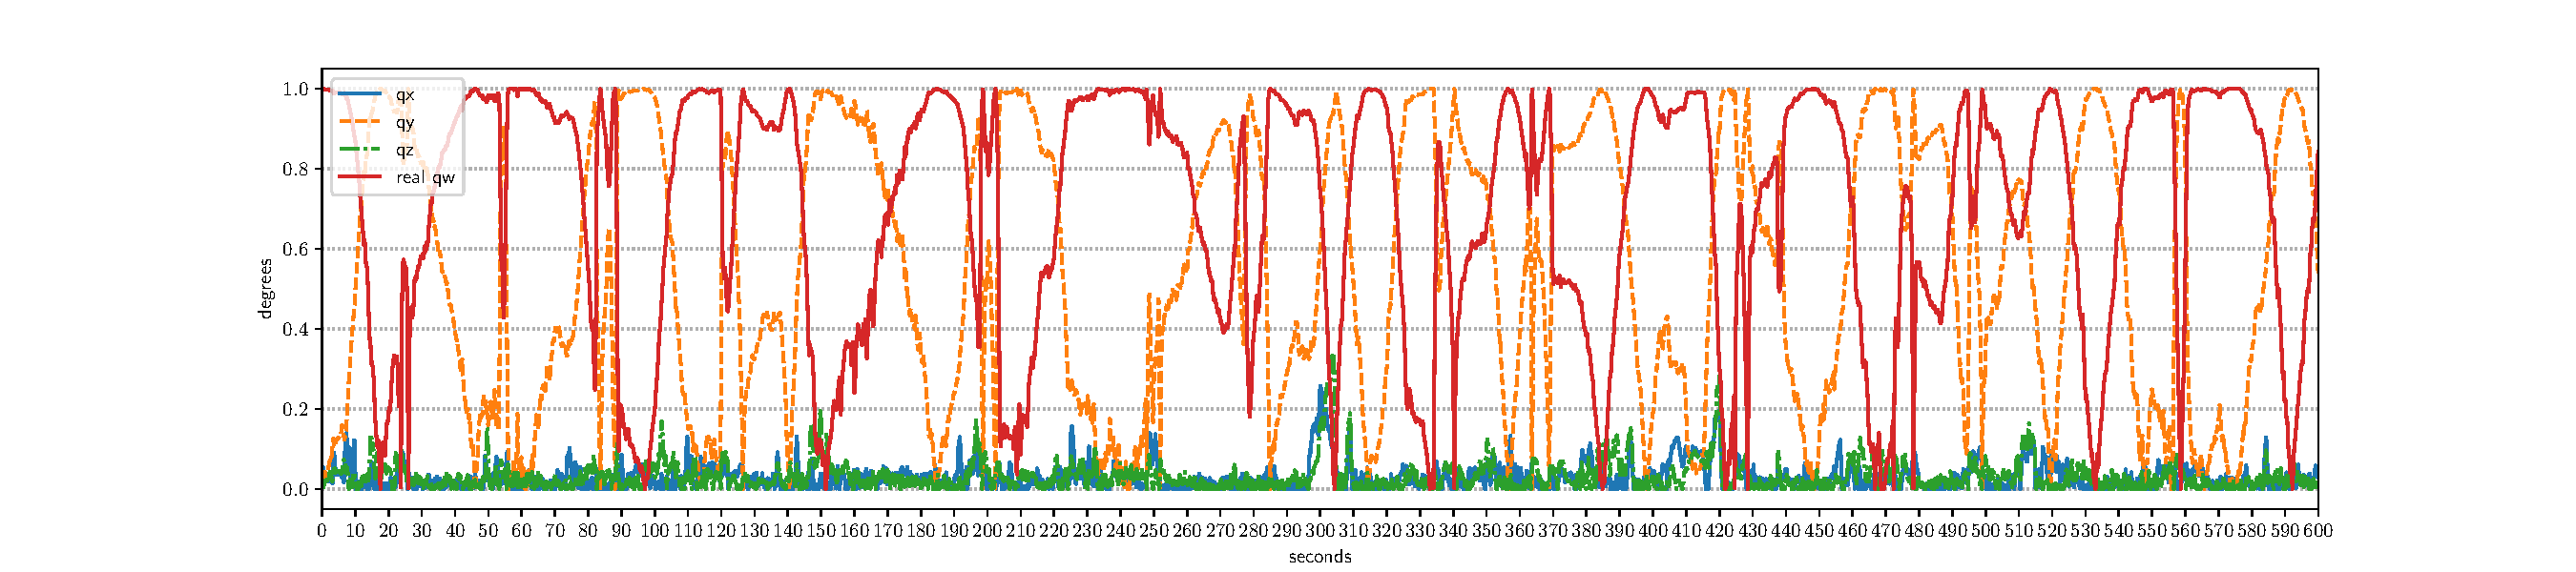
\includegraphics[width=1\textwidth, keepaspectratio]{gfx/Fig-1556-quaternions_flipped.pdf}
		\caption{\label{fig:norm_data} Quaternions from 6-DoF dataset's flipped if their real part is negative}
	\end{center}
\end{figure}

The figure \ref{fig:compare} represents quaternions of the original interpolated dataset on the upper part of the plot and the normalized flipped quaternions on the lower part of the plot. The quaternion's components were flipped only if the if their real part became negative. Different to figure \ref{fig:norm_data} the limit of y-axis is set to [-1, 1] on figure  \ref{fig:compare} so that the result of inverting of quaternion is easy co compare to original data.  Figure \ref{fig:norm_data} shows plotted data with length of 20 seconds in range 162 - 182 s from both datasets.

\begin{figure}[htb]
	\begin{center}
		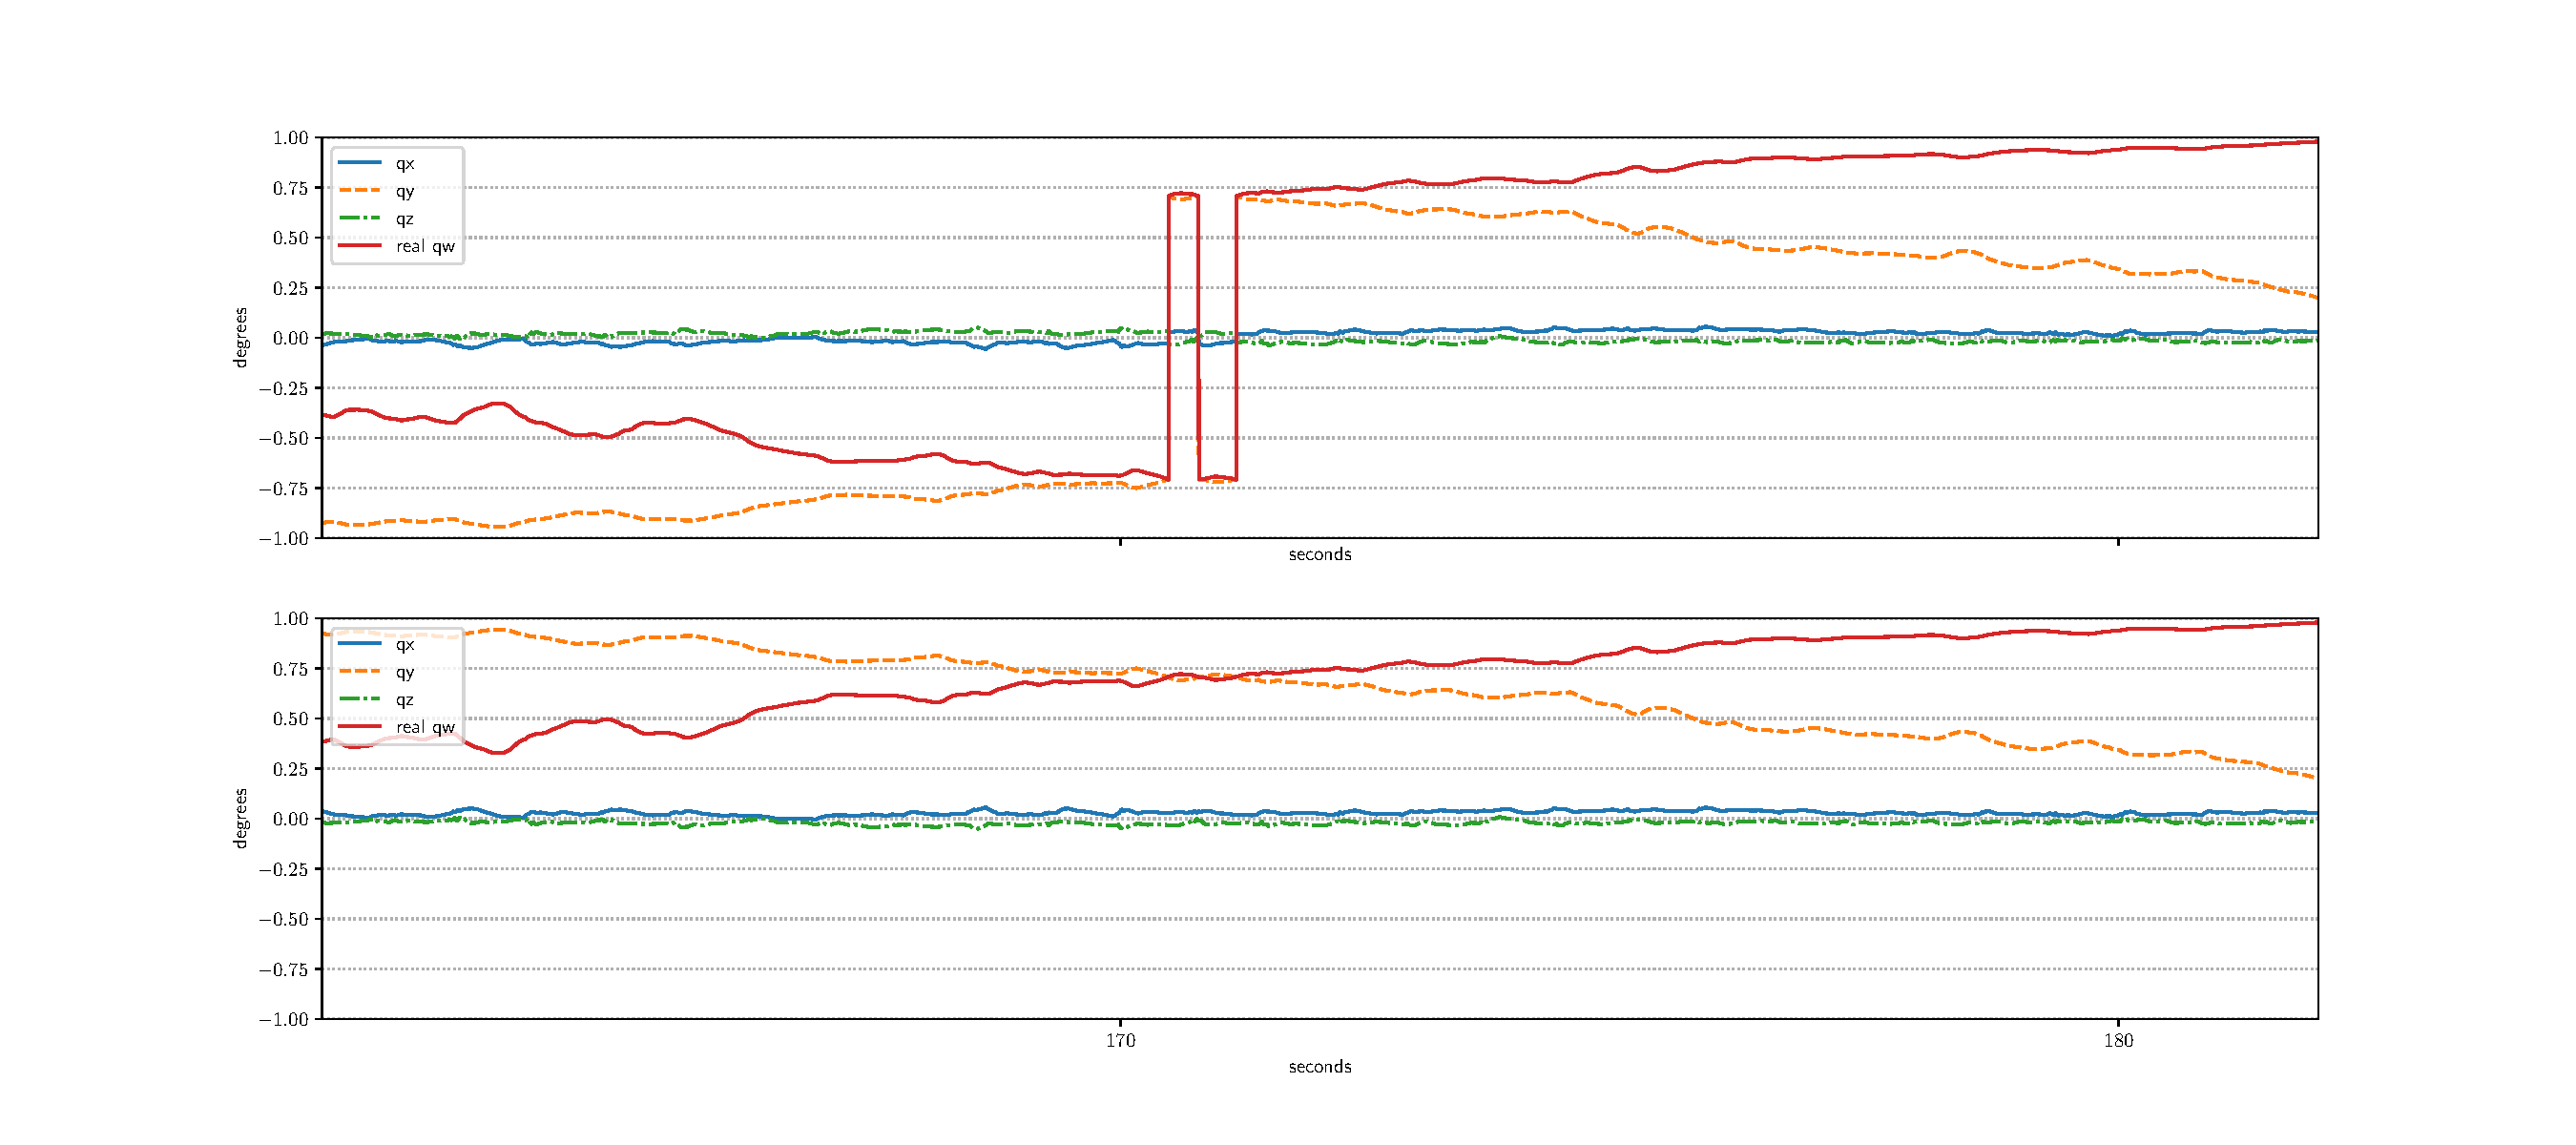
\includegraphics[width=1\textwidth, keepaspectratio]{gfx/Fig-1556-compare.pdf}
		\caption{\label{fig:compare} Quaternions from 6-DoF dataset's flipped if their real part is negative}
	\end{center}
\end{figure}



\subsection{Data Exploration}
\label{sec:design:dataset:explor}


!! Data analysis AVG linear velocity position, plots 

We can make two important observations based on the sample trace: firstly, the viewer rarely moves along the y-axis (except for the time period between 38-42 s during which the viewer probably sat down and stood back up), which is understandable since it requires more effort to crouch down and stand up. Secondly, the orientation changes are typically due to yaw movements, whereas the magnitude of changes due to roll and pitch movements are much smaller. Our observations are also confirmed by visual inspection of the other recorded traces.


\section{Neural Network}
\label{sec:design:nn}

\subsection{Network architecture}
\label{sec:design:nn:architecture}

\subsection{Network input}
\label{sec:design:nn:input}


\section{Training methods}
\label{sec:design:train}
